\documentclass[conference]{IEEEtran}
\IEEEoverridecommandlockouts
% The preceding line is only needed to identify funding in the first footnote. If that is unneeded, please comment it out.

\usepackage[T1]{fontenc}
\usepackage[utf8]{inputenc}
\usepackage{lmodern}

\usepackage{cite}
\usepackage{amsmath,amssymb,amsfonts}
\usepackage{algorithmic}
\usepackage{graphicx}
\usepackage{textcomp}
\usepackage{xcolor}
\usepackage{url}
\usepackage{datetime}
\usepackage{microtype}

\newdateformat{schoolyear}{%
  \ifthenelse{\month > 9} % If current month is October or later
    {\the\year/\the\numexpr\year+1-2000\relax} % Show current year / next year (last two digits)
    {\the\numexpr\year-1\relax/\the\numexpr\year-2000\relax} % Show previous year / current year (last two digits)
}

\def\BibTeX{{\rm B\kern-.05em{\sc i\kern-.025em b}\kern-.08em
    T\kern-.1667em\lower.7ex\hbox{E}\kern-.125emX}}
\usepackage{parskip}
\usepackage[hidelinks]{hyperref}





\begin{document}

\title{Assignment \#1:\\Fingerprint Recognition with NBIS}

\author{

\IEEEauthorblockN{Maša Uhan}
\IEEEauthorblockA{\textit{IBB \schoolyear\today, FRI, UL} \\
    \textit{mu34969@student.uni-lj.si}}
% \and
% \IEEEauthorblockN{Second Author}
% \IEEEauthorblockA{\textit{IBB 22/23, FRI, UL} \\
%     \textit{your.email@you.use.as.an.email.id}}

}

\maketitle

% ########################################
\section{Introduction}
We evaluate fingerprint recognition with the NIST Biometric Image Software (NBIS)~\cite{nbis}: we select a matching threshold and classify fingerprint pairs as \emph{same} or \emph{different finger}, first directly and then only within groups of the same pattern type.

% ########################################
% ########################################
\section{Methodology}
Images are converted from TIFF to PNG, as MINDTCT fails on TIFF. MINDTCT detects minutiae (ridge endings and bifurcations); BOZORTH3 compares two minutiae sets independently of rotation and translation and returns an unnormalised score. All fingerprints are compared with all others; the class is the finger id from the file name. Quality is estimated with NFIQ (1 = best, 5 = worst).

\textbf{Threshold selection.} A pair is classified as \emph{same finger} if its score is at least $t$. We compute the accuracy for every integer $t$ up to the highest score and keep the best (smallest on ties); checking all values avoids stopping at a local maximum.

\textbf{Classification.} Each unordered pair is compared once (no A vs.~A or B vs.~A). We report accuracy (correct / all pairs), false acceptance (FAR) and false rejection rate (FRR). In the second experiment, PCASYS first assigns each fingerprint a type (A, L, R, S, T, W); only pairs of the same type are matched, others are classified as \emph{different finger}.

% ########################################
\section{Experiments}
We use FVC2002 DB1\_B~\cite{fvc2002}: 10 fingers with 8 impressions each ($388\times374$\,px, 500\,dpi optical sensor), giving 3{,}160 unique pairs (280 genuine, 2{,}880 impostor). As instructed, the whole dataset is used for threshold selection and evaluation. NBIS tools use default parameters. PCASYS needs WSQ images of at least $512\times480$\,px, so images are padded with white to $600\times600$ and compressed with \texttt{cwsq} (bitrate 0.75); we use its MLP classifier.

% ########################################
\section{Results and Discussion}
\begin{table}[!h]
\caption{Classification of the 3{,}160 unique pairs with the selected $t=27$. \emph{Matched}: pairs compared with BOZORTH3.}
\begin{center}
\begin{tabular}{lrrrr}
 Experiment & Matched & Acc. [\%] & FAR [\%] & FRR [\%] \\
 \hline
 No types & 3{,}160 & 98.99 & 0.10 & 10.36 \\
 PCASYS types & 1{,}172 & 98.29 & 0.03 & 18.93
\end{tabular}
\label{tab1}
\end{center}
\end{table}

% #################
\subsection{Results}
The best threshold is $t=27$ (Table~\ref{tab1}). Impostor scores lie between 0 and 30 (mean 7.3), genuine ones between 0 and 289 (mean 95.5) (Fig.~\ref{fig:scores}).

\begin{figure}[!h]
\begin{center}
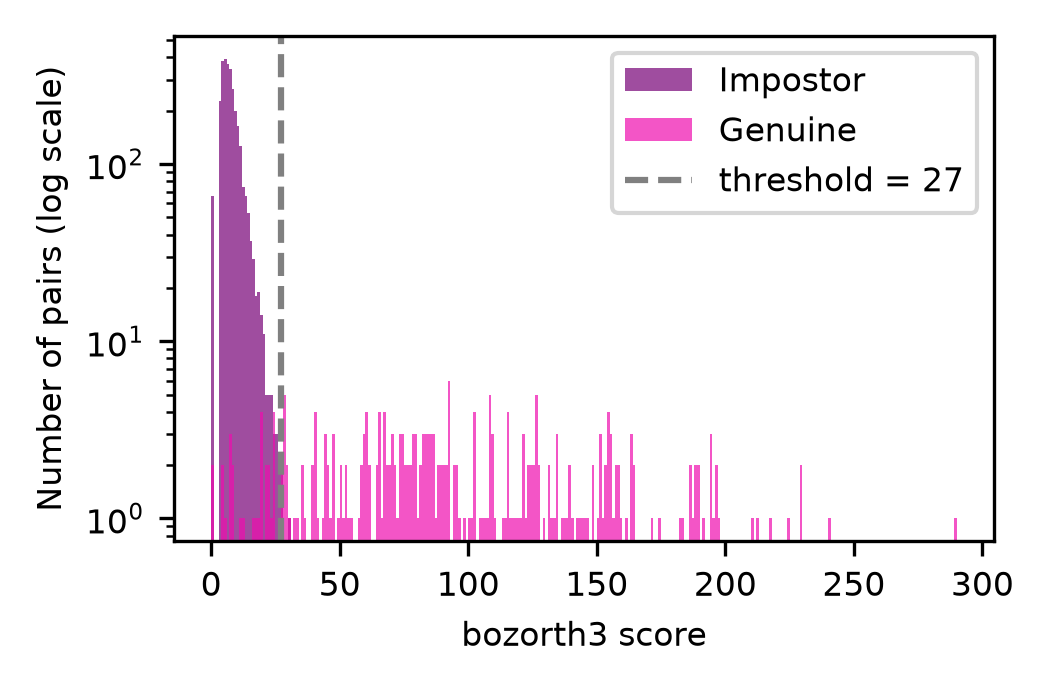
\includegraphics[width=\columnwidth]{figs/genuine_impostor.png}
\end{center}
\caption{BOZORTH3 scores of the 280 genuine and 2{,}880 impostor pairs (log-scale y-axis). The dashed line marks the selected threshold $t=27$.}
\label{fig:scores}
\end{figure}

In the similarity matrix (Fig.~\ref{fig:matrix}) each finger forms a block on the diagonal. NFIQ rates 38 images with quality 1, 35 with 2 and 7 with 3 (Fig.~\ref{fig:quality}).

\begin{figure}[!h]
\begin{center}
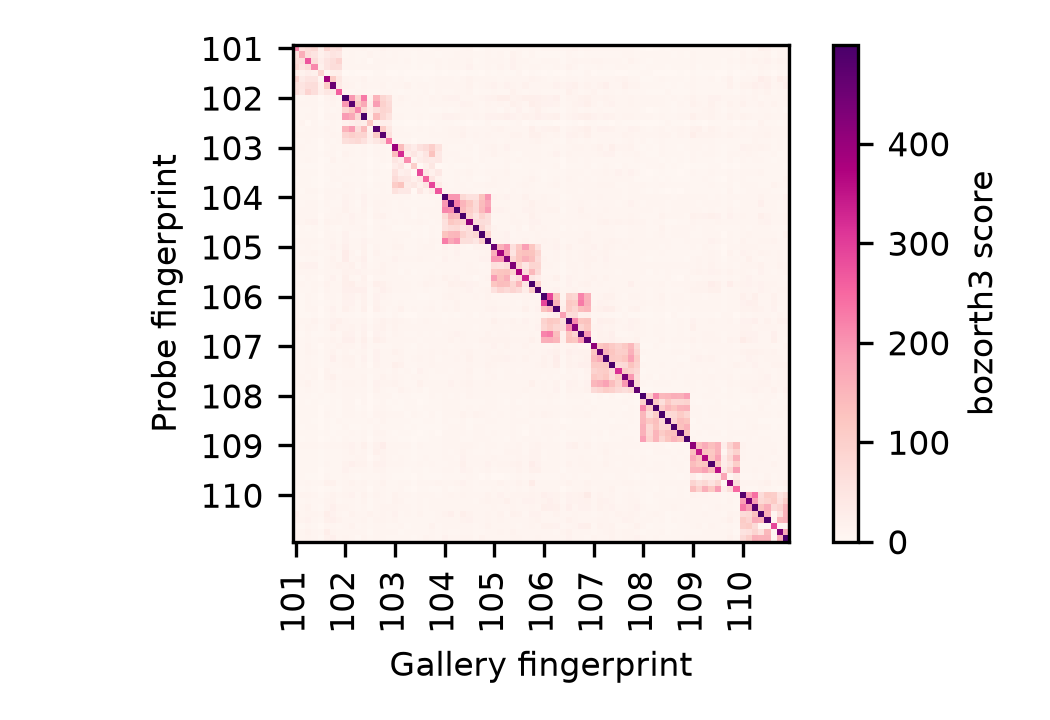
\includegraphics[width=\columnwidth]{figs/similarity_matrix.png}
\end{center}
\caption{Similarity matrix of all $80\times80$ comparisons, sorted by finger. Pale rows inside a block are impressions that match their finger poorly.}
\label{fig:matrix}
\end{figure}

\begin{figure}[!h]
\begin{center}
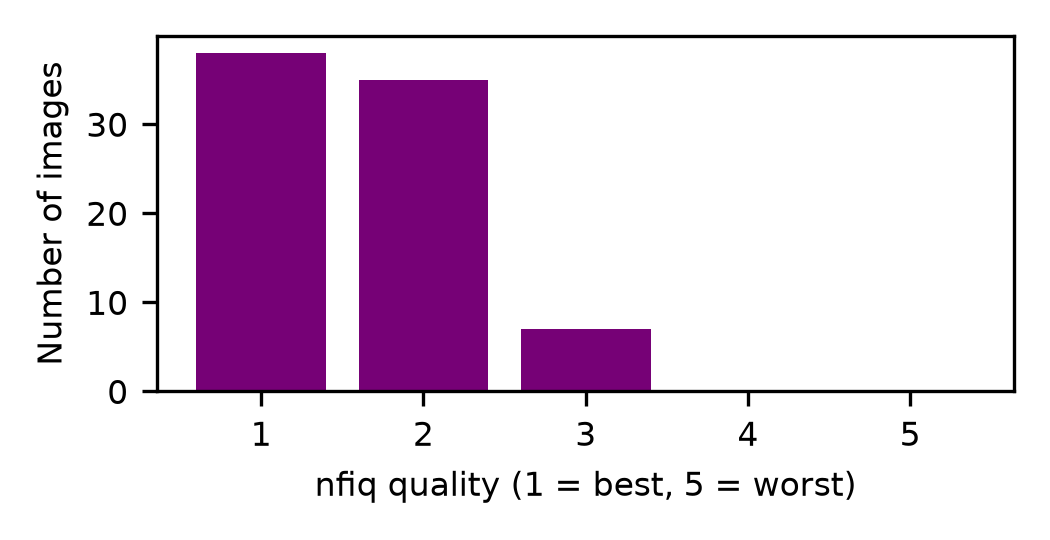
\includegraphics[width=\columnwidth]{figs/quality.png}
\end{center}
\caption{Images per NFIQ quality level (1 = best, 5 = worst).}
\label{fig:quality}
\end{figure}

% #################
\subsection{Discussion}
The classes are imbalanced: rejecting every pair would already give 91.14\% accuracy. Almost all errors are false rejections, linked to low quality: the 7 quality-3 images come from fingers 101, 107 and 109 (four from 109, which has a weak block in Fig.~\ref{fig:matrix}).

With PCASYS, four impressions get a different type than the rest of their finger, so 26 genuine pairs are rejected without matching, nearly doubling the FRR. In exchange, two of three false acceptances disappear and 63\% of comparisons are avoided.

% ########################################
\section{Conclusion}
With $t=27$, chosen by maximising accuracy, pair classification reaches 98.99\% accuracy. Matching within PCASYS types saves 63\% of comparisons at a small accuracy cost, as a wrong type cannot be corrected later. As the threshold was tuned and evaluated on the same small dataset, the results are optimistic.

% ########################################
\bibliographystyle{IEEEtran}
\bibliography{report}

\end{document}
